\documentclass{sigchi}

% Use this command to override the default ACM copyright statement (e.g. for preprints). 
% Consult the conference website for the camera-ready copyright statement.


%% EXAMPLE BEGIN -- HOW TO OVERRIDE THE DEFAULT COPYRIGHT STRIP -- (July 22, 2013 - Paul Baumann)
% \toappear{Permission to make digital or hard copies of all or part of this work for personal or classroom use is 	granted without fee provided that copies are not made or distributed for profit or commercial advantage and that copies bear this notice and the full citation on the first page. Copyrights for components of this work owned by others than ACM must be honored. Abstracting with credit is permitted. To copy otherwise, or republish, to post on servers or to redistribute to lists, requires prior specific permission and/or a fee. Request permissions from permissions@acm.org. \\
% {\emph{CHI'14}}, April 26--May 1, 2014, Toronto, Canada. \\
% Copyright \copyright~2014 ACM ISBN/14/04...\$15.00. \\
% DOI string from ACM form confirmation}
%% EXAMPLE END -- HOW TO OVERRIDE THE DEFAULT COPYRIGHT STRIP -- (July 22, 2013 - Paul Baumann)


% Arabic page numbers for submission. 
% Remove this line to eliminate page numbers for the camera ready copy
% \pagenumbering{arabic}


% Load basic packages
\usepackage{balance}  % to better equalize the last page
\usepackage{graphics} % for EPS, load graphicx instead
\usepackage{times}    % comment if you want LaTeX's default font
\usepackage{url}      % llt: nicely formatted URLs

% llt: Define a global style for URLs, rather that the default one
\makeatletter
\def\url@leostyle{%
  \@ifundefined{selectfont}{\def\UrlFont{\sf}}{\def\UrlFont{\small\bf\ttfamily}}}
\makeatother
\urlstyle{leo}


% To make various LaTeX processors do the right thing with page size.
\def\pprw{8.5in}
\def\pprh{11in}
\special{papersize=\pprw,\pprh}
\setlength{\paperwidth}{\pprw}
\setlength{\paperheight}{\pprh}
\setlength{\pdfpagewidth}{\pprw}
\setlength{\pdfpageheight}{\pprh}

% Make sure hyperref comes last of your loaded packages, 
% to give it a fighting chance of not being over-written, 
% since its job is to redefine many LaTeX commands.
\usepackage[pdftex]{hyperref}
\hypersetup{
pdftitle={MACHINE-ASSISTED COOKING},
pdfauthor={LaTeX},
pdfkeywords={SIGCHI, proceedings, archival format},
bookmarksnumbered,
pdfstartview={FitH},
colorlinks,
citecolor=black,
filecolor=black,
linkcolor=black,
urlcolor=black,
breaklinks=true,
}

% create a shortcut to typeset table headings
\newcommand\tabhead[1]{\small\textbf{#1}}


% End of preamble. Here it comes the document.
\begin{document}

\title{Machine-Assisted Cooking}


%\numberofauthors{1}
%\author{
%  \alignauthor Miriam Cha, Michelle Deng, and Melih Elibol\\
%    \affaddr{Harvard University}\\
%    \affaddr{Cambridge, MA 02138}\\
%    \email{\{miriamcha, michelledeng, melihelibol\}@g.harvard.edu}\\
%}

\numberofauthors{3}
\author{
  \alignauthor Miriam Cha\\
    \affaddr{Harvard University}\\
    \affaddr{Cambridge, MA 02138}\\
    \email{miriamcha@fas.harvard.edu}\\
  \alignauthor Michelle Deng\\
    \affaddr{Harvard College}\\
    \affaddr{Cambridge, MA 02138}\\
    \email{mdeng@college.harvard.edu}\\
  \alignauthor Melih Elibol\\
    \affaddr{Harvard Extension School}\\
    \affaddr{Cambridge, MA 02138}\\
    \email{elibol@fas.harvard.edu}\\
}

\maketitle

\begin{abstract}
In this paper we describe the formatting requirements for
SIGCHI Conference Proceedings, and this sample file
offers recommendations on writing for the worldwide
SIGCHI readership. Please review this document even if
you have submitted to SIGCHI conferences before, some
format details have changed relative to previous years.
\end{abstract}

\keywords{
	Guides; instructions; author's kit; conference publications;
	keywords should be separated by a semi-colon. \newline
	\textcolor{red}{Optional section to be included in your final version, 
  but strongly encouraged.}
}

\category{H.5.m.}{Information Interfaces and Presentation (e.g. HCI)}{Miscellaneous}

%See: \url{http://www.acm.org/about/class/1998/}
%for more information and the full list of ACM classifiers
%and descriptors. \newline
%\textcolor{red}{Optional section to be included in your final version, 
%but strongly encouraged. On the submission page only the classifiers’ 
%letter-number combination will need to be entered.}

\section{Introduction}
Cooking can be a source of enjoyment and pride and a forum for creative experimentation. Compared to prepackaged and most restaurant meals, homemade meals can be healthier and cheaper. However, developing the proper skills to cook with confidence takes time and patience. The tools, ingredients, motor skills, effective use of heating/cooling appliances, pressures of precise timing, importance of precise timing, as well as several other factors may seem overwhelming to novices. In a world where people are on the run, prepackaged meals, restaurants, and near-instant food delivery are appealing alternatives to cooking.

Many people perceive cooking as stressful and time-consuming or simply not worth learning. We believe the difficulties involved in cooking are primarily due to cognitive overload. Getting your first meal right is almost impossible without help, and failure may discourage people from trying again. There are few resources that currently exist which help mitigate the cognitive load experienced by first-time cooks. For instance, printed cookbooks increase cognitive load, because ingredients and instructions must be memorized in order to cook without interruption. Cooking blogs (e.g., \cite{cooking_classy, allrecipes}) provide plenty of recipes and guides, but these sources are merely digital versions of printed cookbooks. Cook Assistant Lite is one cellphone application that has made cooking interactive \cite{cook_lite}, but the application requires the user to continually interact with the application, which leads to even more interruptions while cooking.

In this paper, we propose a digital cooking assistant design for novice cooks. Our design focuses on the following points:
\begin{itemize}
\item	Mitigate interruptions that are due to overutilization of visual input (necessary visual observations while cooking and having to continually read something to determine what to do next) and motor functions (hands are used for cooking and clicking through applications or scrolling on a blog).
\item Mitigate cognitive overload that is due to the physical and temporal demands of cooking, which are exacerbated by the memorization of ingredients and instructions.
\item Make instructions in recipes more accessible, teach users new cooking techniques, and help users decide what to make with the ingredients they already have at home.
\end{itemize}

Features of our design include text-to-speech instruction; timers for managing multiple simultaneous tasks; reminders to check oven and stove temperatures; easy-to-read interfaces that display one step at a time with large pictorial, audio, and/or video aids, somewhat reminiscent of turn-by-turn navigation of a GPS; and lifelines to contact other users who have previously tried the recipe.

Our approach is user-centered. We survey both novice and expert cooks in order to identify key differences between skill levels. For instance: What do novice cooks find most difficult about cooking? What prevents them from cooking more often? What motivates experts to cook? Survey results inform our design of several paper-based interfaces. We then conduct a round of in-person questionnaires to obtain feedback on multiple paper-based designs, which help to identify prominent features and issues with each design. We show multiple designs in parallel to each participant. After incorporating feedback on paper prototypes, we implement the digital design leveraging the recipe API BigOven \cite{api_oven}. To assess the quality of our digital prototype(s), we conduct a within-subject experiment, comparing user performance on cooking recipes with and without our prototype(s). During the performance phase, we collect qualitative data by observation. After each cooking session, we ask the user to assess their cooking experience based on the following factors (NASA Task Load Index): mental demand, physical demand, temporal demand, performance, effort, and frustration. Finally, through further user testing and design/development iteration, our final product embodies the features that help first-time and novice cooks succeed in their cooking adventures.

\section{Related Work}
Cognitive theory has been extensively studied in the field of instructional interface
design. The majority of work is based on Baddeley?s canonical model of working
memory as a limited buffer for visual and auditory information [a]. When the buffer is
overloaded, possibly by performing complex tasks that involve an ordered series of
physical and mental activities, new information can fail to be processed [a, b]. Mayer
(2005) expands Baddeley?s model to form a cognitive theory of multimedia learning [c,
d]. In his model, information processing is divided into a verbal (not necessarily
auditory) channel and a visual channel. Again, each channel has a fixed informationprocessing
capacity and can be overloaded. Mayer presents a series of principles for
designing instructional multimedia aimed to reduce cognitive effort required from the
learner for one or more channels [c].
Over the last decade, similar principles have often been used in the design of
multimedia systems for academic or conceptual instruction, e.g., Moons and De Backer
(2011), or Wong et al., (2012). However, unlike academics, most activities, cooking
included, require less intellectual effort but require coordination of motion and
sensation. The requirements on the channels of information processing thus differ.
Paas and Sweller (2011) argue that "biologically primary" skills passed through evolution
require less cognitive effort than explicitly learned, often culturally driven "secondary"
skills. Based on time of historical emergence, movement-based activities like sports and
cooking should be more primary than many fields of academics. On the other hand,
Post et al. (2013) find that gesturing while watching grammar-instruction animations
interferes with learning, and grammar could arguably be a primary skill. Moreover,
interference from over loading could be bidirectional, for it is well established that
secondary in-vehicle activities such as phoning or texting compromises drivers? ability to
react to road conditions, leading to injuries and fatalities [f].
Several questions arise, yet few studies have directly investigated the cognitive load
effects of teaching tools in non-academic situations. In a rare study, Khacharem et al.
(2014) investigate the cognitive load effects of animations used for soccer instruction
and find that novice players process both static images better than animations and
slow animations better than fast ones, whereas expert players learn more effectively
with fast animations. Their results suggest that speed and motion from instruction
alone can add additional tolls on cognitive load, but these instructions were conveyed
offline, as opposed to during gameplay.
The body of literature on cooking is similarly patchy. Recipe recommendation and
generation are well documented in the literature [y, u, o]; many such systems have
been built (e.g., gg) but do not assist users in making the recipe. Meanwhile, little or no
research investigates the cognitive load of cooking, and few systems seek to address
the possible overload. Kraft?s iFood Assistant [q] and Quasar Computing?s Cook
Assistant Lite [j] seem to share our goals, but their design choices and user test results,
if any, are not documented.

\section{Field Visit \#1: Blah}

On each page your material (not including the page number) should fit
within a rectangle of 18 x 23.5 cm (7 x 9.25 in.), centered on a US
letter page, beginning 1.9 cm (.75 in.) from the top of the page, with
a .85 cm (.33 in.) space between two 8.4 cm (3.3 in.) columns.  Right
margins should be justified, not ragged. Beware, especially when using
this template on a Macintosh, Word can change these dimensions in
unexpected ways. Please be sure that your PDF is US letter and not
A4. If your PDF or paper are formatted for A4, the submission will be
returned to you to fix.

\subsection{Contextual Studies}
blah

\subsection{Paper Prototypes}
blah

\section{Field Visit \#2: Blah}

Prepare your submissions on a word processor or typesetter.  Please
note that page layout may change slightly depending upon the printer
you have specified.  \LaTeX\ sometimes will create overfull lines
that extend into columns.  To attempt to combat this, the .cls
file has a command, {\textbackslash}sloppy, that essentially asks
\LaTeX\ to prefer underfull lines with extra whitespace.  For more
details on this, and info on how to control it more finely, check out
{\url{http://www.economics.utoronto.ca/osborne/latex/PMAKEUP.HTM}}.

\subsection{Contextual Studies}
blah

\subsection{Prototype Evaluation}

\section{Field Visit \#3: Blah}

Your paper's title, authors and affiliations should run across the
full width of the page in a single column 17.8 cm (7 in.) wide.  The
title should be in Helvetica 18-point bold; use Arial if Helvetica is
not available.  Authors' names should be in Times Roman 12-point bold,
and affiliations in Times Roman 12-point.  For more than three authors,
you may have to place some address information in a footnote, or in a named
section at the end of your paper. Please use full international addresses and
telephone dialing prefixes.  Leave one 10-pt line of white space below the last
line of affiliations.

\subsection{Design Observations}

\subsubsection{Interactive Icons}

\subsubsection{Speech Processing}

\section{Related Work}

Every submission should begin with an abstract of about 150 words,
followed by a set of keywords. The abstract and keywords should be
placed in the left column of the first page under the left half of the
title. The abstract should be a concise statement of the problem,
approach and conclusions of the work described.  It should clearly
state the paper's contribution to the field of HCI.

The first set of keywords will be used to index the paper in the
proceedings. The second set are used to catalogue the paper in the ACM
Digital Library. The latter are entries from the ACM Classification
System~\cite{acm_categories}.  In general, it should only be necessary
to pick one or more of the H5 subcategories, see
\url{http://www.acm.org/class/1998/ccs98.html}

\section{Conclusions and Future Work}

Please use a 10-point Times Roman font or, if this is unavailable,
another proportional font with serifs, as close as possible in
appearance to Times Roman 10-point. The Press 10-point font available
to users of Script is a good substitute for Times Roman. If Times
Roman is not available, try the font named Computer Modern Roman. On a
Macintosh, use the font named Times and not Times New Roman. Please
use sans-serif or non-proportional fonts only for special purposes,
such as headings or source code text.

\begin{figure}[!h]
\centering
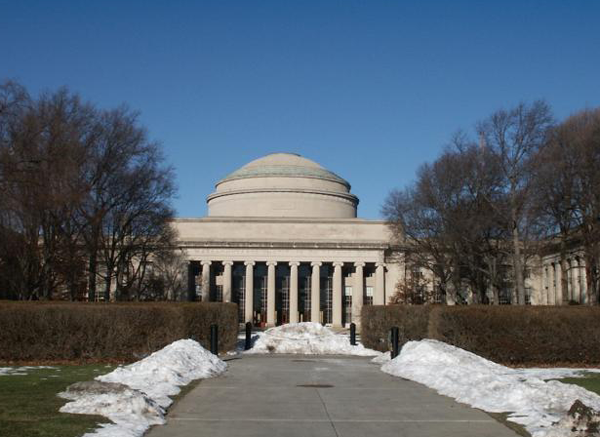
\includegraphics[width=0.9\columnwidth]{Figure1}
\caption{With Caption Below, be sure to have a good resolution image
  (see item D within the preparation instructions).}
\label{fig:figure1}
\end{figure}

\subsection{References and Citations}

Use a numbered list of references at the end of the article, ordered
alphabetically by first author, and referenced by numbers in brackets
\cite{ethics,
  Klemmer:2002:WSC:503376.503378,
  Mather:2000:MUT,
  Zellweger:2001:FAO:504216.504224}. For
papers from conference proceedings, include the title of the paper and
an abbreviated name of the conference (e.g., for Interact 2003
proceedings, use \textit{Proc. Interact 2003}). Do not include the
location of the conference or the exact date; do include the page
numbers if available. See the examples of citations at the end of this
document. Within this template file, use the \texttt{References} style
for the text of your citation.

Your references should be published materials accessible to the
public.  Internal technical reports may be cited only if they are
easily accessible (i.e., you provide the address for obtaining the
report within your citation) and may be obtained by any reader for a
nominal fee.  Proprietary information may not be cited. Private
communications should be acknowledged in the main text, not referenced
(e.g., ``[Robertson, personal communication]'').

\begin{table}
  \centering
  \begin{tabular}{|c|c|c|}
    \hline
    \tabhead{Objects} &
    \multicolumn{1}{|p{0.3\columnwidth}|}{\centering\tabhead{Caption --- pre-2002}} &
    \multicolumn{1}{|p{0.4\columnwidth}|}{\centering\tabhead{Caption --- 2003 and afterwards}} \\
    \hline
    Tables & Above & Below \\
    \hline
    Figures & Below & Below \\
    \hline
  \end{tabular}
  \caption{Table captions should be placed below the table.}
  \label{tab:table1}
\end{table}



\section{Conclusion}

\section{Acknowledgments}

We thank CHI, PDC and CSCW volunteers, and all publications support
and staff, who wrote and provided helpful comments on previous
versions of this document.  Some of the references cited in this paper
are included for illustrative purposes only.  \textbf{Don't forget
to acknowledge funding sources as well}, so you don't wind up
having to correct it later.

% Balancing columns in a ref list is a bit of a pain because you
% either use a hack like flushend or balance, or manually insert
% a column break.  http://www.tex.ac.uk/cgi-bin/texfaq2html?label=balance
% multicols doesn't work because we're already in two-column mode,
% and flushend isn't awesome, so I choose balance.  See this
% for more info: http://cs.brown.edu/system/software/latex/doc/balance.pdf
%
% Note that in a perfect world balance wants to be in the first
% column of the last page.
%
% If balance doesn't work for you, you can remove that and
% hard-code a column break into the bbl file right before you
% submit:
%
% http://stackoverflow.com/questions/2149854/how-to-manually-equalize-columns-
% in-an-ieee-paper-if-using-bibtex
%
% Or, just remove \balance and give up on balancing the last page.
%
\balance

\section{References format}
References must be the same font size as other body text.
% REFERENCES FORMAT
% References must be the same font size as other body text.

\bibliographystyle{acm-sigchi}
\bibliography{sample}
\end{document}
